% =========================================================================== %
% Preamble                                                                    %
% =========================================================================== %

\documentclass[12pt, dvipsnames, aspectratio=169]{beamer}
%\documentclass[12pt, dipsnames, notes=only]{beamer}

\usepackage[utf8]{inputenc}
\usepackage{beamerthemesimple}

\date{February 24$^{th}$, 2021}
\title{GRIFFIN\@: Guarding Control Flows Using Intel Processor Trace}
\author{William Findlay}
\institute{Carleton University\\\href{mailto:will@ccsl.carleton.ca}{\ttfamily will@ccsl.carleton.ca}}

\usepackage{csquotes}
\usepackage{booktabs}

% Center floats by default
\makeatletter
\g@addto@macro\@floatboxreset{\centering}
\makeatother

\usepackage{listings}

\lstnewenvironment{listing}[1][]{\lstset{#1}}{}

\definecolor[named]{red}{HTML}{A4031F}
\definecolor[named]{blue}{HTML}{0071B2}
\definecolor[named]{orange}{HTML}{E59C00}
\definecolor[named]{green}{HTML}{009E73}
\definecolor[named]{purple}{HTML}{88498F}
\definecolor[named]{dark-grey}{HTML}{515151}
\definecolor[named]{grey}{HTML}{797979}

\colorlet{listing-basic}{dark-grey}
\colorlet{listing-keyword}{blue}
\colorlet{listing-keyword-2}{orange}
\colorlet{listing-keyword-3}{purple}
\colorlet{listing-comment}{grey}
\colorlet{listing-string}{green}

% Set default listings style
\lstdefinestyle{listingstyle}{
    basicstyle       = {\ttfamily\color{listing-basic}\lst@ifdisplaystyle\scriptsize\fi},
    keywordstyle     = {\color{listing-keyword}\bfseries},
    keywordstyle     = {[2]\color{listing-keyword-2}\bfseries},
    keywordstyle     = {[3]\color{listing-keyword-3}\bfseries},
    identifierstyle  = {\color{listing-keyword-3}\bfseries},
    sensitive        = true,
    commentstyle     = {\color{listing-comment}},
    stringstyle      = {\color{listing-string}},
    showstringspaces = false,
    columns          = fullflexible,
    keepspaces       = true,
    literate         = {~}{$\sim$}{1},
    escapeinside     = {!@}{@!}
}
\lstset{style=listingstyle}

% x64 asm language
\lstdefinelanguage
   {x64}     % add a "x64" dialect of Assembler
   [x86masm]{Assembler} % based on the "x86masm" dialect
   % with these extra keywords:
   {morekeywords={cdqe,cqo,cmpsq,cmpxchg16b,jrcxz,lodsq,movsxd, %
                  popfq,pushfq,scasq,stosq,iretq,rdtscp,swapgs, %
                  leaq,movq,movl,pause,lfence, %
                  rax,rdx,rcx,rbx,rsi,rdi,rsp,rbp,rip, %
                  r8,r8d,r8w,r8b,r9,r9d,r9w,r9b, %
                  r10,r10d,r10w,r10b,r11,r11d,r11w,r11b, %
                  r12,r12d,r12w,r12b,r13,r13d,r13w,r13b, %
                  r14,r14d,r14w,r14b,r15,r15d,r15w,r15b}} % etc.

% Define "none" language for listings
\lstdefinelanguage{none}{
  identifierstyle = {\color{listing-basic}}
}

\setbeamertemplate{section in toc}[sections numbered]

\hypersetup{
    colorlinks = true,
    linkcolor  = .,
    urlcolor   = blue,
    citecolor  = blue,
}
\urlstyle{tt}

\newcommand{\fullframegraphic}[1]{%
    {%
        \setwatermark{}
        \usebackgroundtemplate{\includegraphics[width=\paperwidth]{#1}}
        \begin{frame}[plain]
        \end{frame}
    }
}

\newcommand\ufootnote[1]{%
    \begingroup
        \renewcommand\thefootnote{}\footnote{\hspace{-1.8em}#1}%
        \addtocounter{footnote}{-1}%
    \endgroup
}

% Table of Contents for sections
\AtBeginSection[]
{
    \begingroup
    \setwatermark{}
    \begin{frame}[c, noframenumbering, plain]
        \begin{center}
        \fontsize{36}{42} \selectfont \bfseries \color{destacado} \insertsection%
        \end{center}
    \end{frame}
    \endgroup
}

\usepackage{biblatex}
\bibliography{refs.bib}
\renewcommand*{\bibfont}{\footnotesize}

\PassOptionsToPackage{hyphens}{url}
%\setcounter{biburllcpenalty}{1}
%\setcounter{biburlucpenalty}{1}
%\setcounter{biburlbigbreakpenalty}{2}
%\setcounter{biburlbreakpenalty}{1}

\usepackage{appendixnumberbeamer}

\makeatletter
\g@addto@macro{\UrlNoBreaks}{\do:}
\g@addto@macro{\UrlBreaks}{\do/}
\makeatother

\newenvironment{nscenter}
 {\parskip=0pt\par\nopagebreak\centering}
 {\par\noindent\ignorespacesafterend}

\let\lsi\lstinline%
\newcommand{\code}[1]{\lsi[language=c]|#1|}

\usepackage{svg}
\usepackage{mathtools}
\usepackage[normalem]{ulem}

\newcommand{\todo}[1]{{\color{orange}[#1]}}
\providecommand{\etal}{{\textit{et al\@.}}}

\newcommand{\red}[1]{{\color{red}#1}}
\newcommand{\orange}[1]{{\color{orange}#1}}
\newcommand{\blue}[1]{{\color{blue}#1}}
\newcommand{\purple}[1]{{\color{purple}#1}}
\newcommand{\green}[1]{{\color{green}#1}}

% =========================================================================== %
% Document                                                                    %
% =========================================================================== %

\begin{document}

% Optional watermark
\setwatermark[hoffset=0.3cm, voffset=0.3cm]{
\includegraphics[width=8cm]{figs/logos/griffin.png}}

% Title page
\begin{frame}[noframenumbering, plain]
  \titlepage%
  \vfill
  \vspace{4em}
  {\footnotesize COMP5900X Discussion Lead}
\end{frame}

%\begin{frame}[c, noframenumbering, plain]{Outline of this Talk}
%    \tableofcontents
%\end{frame}
%
%\section{Untitled Section}

\begin{frame}[c]{Paper Overview}{}
  {\bf Title}
  \begin{itemize}
    \item \enquote{GRIFFIN\@: Guarding Control Flows Using Intel Processor Trace}
    \item New online CFI mechanism based on Intel Processor Trace
  \end{itemize}

  \vfill
  {\bf Authors}
  \begin{itemize}
    \item Xinyang Ge, Weidong Cui, Trent Jaeger\footnote{You might know Trent Jaeger from his excellent OS security textbook~\cite{jaeger2008_os_security}}
    \item Microsoft Research, Pennsylvania State University
  \end{itemize}

  \vfill
  {\bf Venue}
  \begin{itemize}
    \item ASPLOS 2017
    \item Architectural Support for Programming Languages and Operating Systems
    \item Recognized as a flagship conference in hardware / OS design
  \end{itemize}
\end{frame}

\begin{frame}[c]{Goals}{}
  {\bf Problem Statement}
  \begin{itemize}
    \item Attackers can abuse memory corruption vulnerabilities to mount code reuse attacks
    \begin{itemize}
      \item Often bypassing existing defences, such as DEP
    \end{itemize}
    \item Defenders can use CFI defences to mitigate code reuse attacks
    \begin{itemize}
      \item Most existing CFI defences are software-only
      \item Hardware-backed CFI can offer better performance, security, flexibility
    \end{itemize}
  \end{itemize}

  \vfill
  {\bf Claims / Contributions}
  \begin{itemize}
    \item First CFI mechanism to use Intel PT
    \begin{itemize}
      \item Performance is comparable to the fastest software-only CFI, but with better security
    \end{itemize}
    \item Multiple policy granularities for flexibility (performance vs security at runtime)
    \item Potential performance improvements re.~Intel PT design
  \end{itemize}
\end{frame}

\begin{frame}[c]{Threat Model and Assumptions}{}
  {\bf \color{blue} Trusted}
  \begin{itemize}
    \item The protected programs themselves (assumed benign)
    \begin{itemize}
      \item But they might contain logic errors / memory corruption vulnerabilities
    \end{itemize}
    \item The operating system (including \blue{all ring 0 code})
    \begin{itemize}
      \item Otherwise attacker could subvert / disable / bypass Griffin
    \end{itemize}
  \end{itemize}

  \vfill
  {\bf \color{orange} Not Trusted}
  \begin{itemize}
    \item Input into protected applications
    \begin{itemize}
      \item Could be used for \orange{memory corruption attacks}
    \end{itemize}
  \end{itemize}

  \vfill
  {\bf \color{green} Assumptions}
  \begin{itemize}
    \item Protected applications implement $W\oplus X$ defence
    \begin{itemize}
      \item Application cannot modify its own code
      \item Application cannot map pages as both writable and executable
    \end{itemize}
  \end{itemize}
\end{frame}

\begin{frame}[c]{Motivation}{}
  \begin{itemize}
    \item Existing CFI space is dominated by {\bf software-only solutions}
    \begin{itemize}
      \item These are generally either {\bf very slow} or {\bf very inflexible}
    \end{itemize}

    \vfill
    \item Hardware-backed CFI hasn't been explored as much
    \begin{itemize}
      \item Existing proposals incur {\bf prohibitive overhead} or offer {\bf incomplete protection}
      \item There is room in the literature to explore newer and more effective hardware-backed solutions
    \end{itemize}

    \vfill
    \item Intel Processor Trace (PT) presents an opportunity to revisit hardware-backed CFI
    \begin{itemize}
      \item Very performant (only 5\% base overhead)
      \item Typically used for {\bf offline debugging} and {\bf provenance}
      \item Repurposing it for {\bf online} CFI requires some extra work (Griffin)
    \end{itemize}
  \end{itemize}
\end{frame}

\section{Background}

\begin{frame}[c]{Memory Corruption / Code Reuse Attacks}{}
\begin{center}
  \color{black}%
  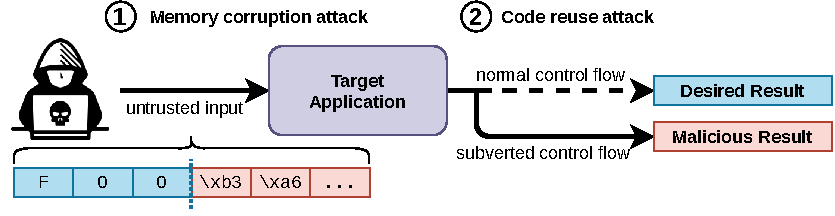
\includegraphics[width=0.8\columnwidth]{figs/memory_corruption.pdf}
\end{center}

\vfill
\begin{itemize}
  \item Memory corruption attack (e.g.~buffer overflow, use-after-free)
  \item Code reuse attack (e.g.~ROP, JOP, ret2libc)
  \item The point is to achieve some attacker goal by subverting normal control flow
  \begin{itemize}
    \item Spawn a shell, write to a sensitive file, disable DEP, etc.
  \end{itemize}
  \item Some defences target the memory corruption step, others target the code reuse step
\end{itemize}
\end{frame}

\begin{frame}[c]{Control Flow Integrity: Overview}{}
{\bf The Basic Idea}
\begin{itemize}
  \item Identify correct code paths for an application $\rightarrow$ control flow graph (CFG)
  \item Enforce correct code paths at runtime (i.e.~they must follow the CFG)
  \item Control flow integrity can stop (many) code reuse attacks
  \begin{itemize}
    \item Depends on sophistication of the attack, granularity of CFI policy
    \item It at least significantly raises the bar for attackers
  \end{itemize}
\end{itemize}

\vfill
{\bf Software CFI Categories}
\begin{enumerate}
  \item Compile-time instrumentation
  \item Static binary instrumentation
  \item Runtime instrumentation
\end{enumerate}
\end{frame}

% FIXME/TODO: Verify the following three slides for accuracy

\begin{frame}[c]{Compile-Time Instrumentation}{}
  {\bf Overview}
  \begin{itemize}
    \item Extend compiler to generate correct CFG for compiled programs
    \item Enforce CFI in language runtime (here, runtime $\equiv$ code you did not write)
  \end{itemize}

  \vfill
  {\bf \blue{Benefits}}
  \begin{itemize}
    \item More efficient than other methods
    \item Easy to capture stateful control flow in CFG model
  \end{itemize}

  \vfill
  {\bf \red{Drawbacks}}
  \begin{itemize}
    \item Bound to specific language, toolchain
    \item CFI enforcement is fixed at compile time (no flexibility)
  \end{itemize}
\end{frame}

\begin{frame}[c]{Static Binary Instrumentation}{}
  {\bf Overview}
  \begin{itemize}
    \item Use static analysis to generate a CFG for an existing binary
    \item Similar to compile-time instrumentation but without compiler support
  \end{itemize}

  \vfill
  {\bf \blue{Benefits}}
  \begin{itemize}
    \item Works on existing and legacy applications
    \item Works across multiple languages
  \end{itemize}

  \vfill
  {\bf \red{Drawbacks}}
  \begin{itemize}
    \item Like compile-time, static binary instrumentation is fixed (no flexibility)
    \item Less accurate than compile-time instrumentation
  \end{itemize}
\end{frame}

\begin{frame}[c]{Runtime Instrumentation}{}
  {\bf Overview}
  \begin{itemize}
    \item Instrument the application at runtime and enforce at runtime
    \item Policy can be generated or manually crafted, changed at will
    \item Griffin technically falls into this category, but uses hardware assistance
  \end{itemize}

  \vfill
  {\bf \blue{Benefits}}
  \begin{itemize}
    \item More flexible than the other two categories
    \item Can be enabled/disabled/changed at runtime to balance security/performance
  \end{itemize}

  \vfill
  {\bf \red{Drawbacks}}
  \begin{itemize}
    \item Can be very slow (sometimes order of magnitude slower)
    \item Implementations that are not very slow offer limited protection
  \end{itemize}
\end{frame}

\begin{frame}[c]{Hardware-Assisted CFI}{}
  \begin{itemize}
    \item CFI backed by some underlying hardware technology for tracing control flows
    \begin{itemize}
      \item E.g.~Intel Branch Target Store (BTS), Last Branch Record (LBR), Performance Monitoring Unit (PMU), Intel Processor Trace (PT)
    \end{itemize}

    \vfill
    \item In general, existing implementations either:
    \begin{itemize}
      \item Do not provide complete protection (e.g.~too coarse-grained)
      \item Incur unacceptable overhead (e.g.~too fine-grained)
    \end{itemize}

    \vfill
    \item Griffin explores a way to efficiently use a newer hardware technology for CFI
    \begin{itemize}
      \item Get more complete protection without sacrificing performance, flexibility
      \item Relies on performance optimizations made possible by Intel PT
    \end{itemize}
  \end{itemize}
\end{frame}

\begin{frame}[c]{Intel Processor Trace: Overview}{}
  \begin{itemize}
    \item A new hardware tracing feature supported by all modern Intel CPUs

    \vfill
    \item Originally designed for \textbf{offline debugging}
    \begin{itemize}
      \item Griffin repurposes it for \textbf{online CFI}
    \end{itemize}

    \vfill
    \item Records a \textbf{minimal trace} that can be used to \textbf{reconstruct control flow}

    \vfill
    \item Traces are recorded in a minified format called \textbf{trace packets}
    \begin{itemize}
      \item Trace packets encode \textbf{branch targets} and \textbf{branch-taken indicators}
      \item \textbf{Branch sources} are \textit{not} recorded
      \item Full control flow reconstruction requires trace packets + program binaries
    \end{itemize}

    \vfill
    \item Trace packets are directly stored in contiguous physical memory regions
    \begin{itemize}
      \item Avoids the cost of address translation through the MMU
    \end{itemize}
  \end{itemize}
\end{frame}

\begin{frame}[c]{Intel Processor Trace: Trace Packets}{}
{\bf Packet Generation Enable (PGE)}
\begin{itemize}
  \item IP value at which tracing starts
\end{itemize}

\vfill
{\bf Packet Generation Disable (PGD)}
\begin{itemize}
  \item IP value at which tracing stops
\end{itemize}

\vfill
{\bf Taken Not Taken (TNT)}
\begin{itemize}
  \item Marks up to 6 conditional branches
  \item \texttt{1} $\rightarrow$ taken
  \item \texttt{0} $\rightarrow$ not taken
  \item Specific branches must be inferred from the code + PGE/PGD
\end{itemize}
\end{frame}

\begin{frame}[c]{Intel Processor Trace: Trace Packets}{}
{\bf Target Instruction Pointer (TIP)}
\begin{itemize}
  \item Specifies a target IP for an indirect branch
  \item Specific branch must be inferred from the code + PGE/PGD
\end{itemize}

\vfill
{\bf Flow Update Packet (FUP)}
\begin{itemize}
  \item Specifies a source address for asynchronous events
\end{itemize}

\vfill
{\bf Packet Stream Boundaries (PSB)}
\begin{itemize}
  \item Unique pattern that marks a location in trace output
  \item Can be used as a synchronization point between workers processing the trace
\end{itemize}
\end{frame}

\section{Griffin Design \& Implementation}

\begin{frame}[c]{Design Overview}{}
  \begin{itemize}
    \item Hardware-assisted CFI using Intel PT
    \begin{itemize}
      \item Trace control flow at runtime using Intel PT and compare it to some policy
    \end{itemize}
  \end{itemize}

  \vfill
  \begin{itemize}
    \item Griffin takes PT traces in physical memory + program binary as input
  \end{itemize}

  \vfill
  \begin{itemize}
    \item Disassemble and divide program binary up into {\bf basic blocks}
    \begin{itemize}
      \item A basic block is just a contiguous code region with no jumps, calls, or returns
    \end{itemize}
  \end{itemize}

  \vfill
  \begin{itemize}
    \item Follow traces and match trace packets with basic blocks
    \begin{itemize}
      \item Policy is stored at some offset from code pages in user memory
      \item Look up policy and verify whether CFI has been violated
    \end{itemize}
  \end{itemize}
\end{frame}

\begin{frame}[c]{Design Overview}{}
  \begin{itemize}
    \item Most overhead comes from processing trace logs
    \begin{itemize}
      \item Griffin trades memory usage for performance
      \item Store as much state in memory as possible
    \end{itemize}

    \vfill
    \item Four policy enforcement strategies for balancing security and performance
    \begin{enumerate}
      \item Coarse-grained policy
      \item Fine-grained policy
      \item Stateful policy
      \item Combination policy
    \end{enumerate}

    \vfill
    \item Policy strategy can be switched at runtime according to a trace backlog threshold
    \begin{itemize}
      \item Fall back to a more performant but less secure policy when bottlenecking
      \item Higher threshold $\rightarrow$ lower performance, higher security
      \item Lower threshold $\rightarrow$ higher performance performance, lower security
    \end{itemize}
  \end{itemize}
\end{frame}

\begin{frame}[c]{P1: Coarse-Grained Policy}{}
  \begin{itemize}
    \item Coarse-grained policy deals only in {\bf target addresses for indirect calls}
    \begin{itemize}
      \item This means no need to reconstruct control flow at all (target addresses are just given directly in TIP packets)
      \item Simply mark an indirect target as allowed or not allowed
      \item High performance, lower security
    \end{itemize}

    \vfill
    \item For every code page, store a policy page
    \begin{itemize}
      \item Stored at a constant offset in userspace (+8TB) for fast lookup at runtime
      \item Griffin tracks dynamic linking and maps additional policy pages for libraries
    \end{itemize}

    \vfill
    \item When a program makes an indirect call:
    \begin{enumerate}
      \item Look up the policy page for the target
      \item Check the value at the corresponding address
      \item 1 $\rightarrow$ allowed, 0 $\rightarrow$ denied
    \end{enumerate}
  \end{itemize}
\end{frame}

\begin{frame}[c]{P1: Coarse-Grained Policy}{}
  \begin{center}
    \color{black}
    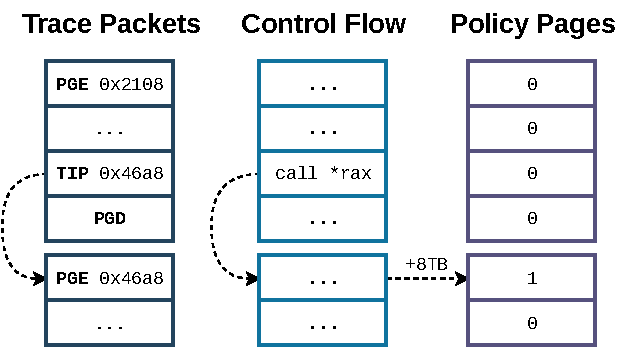
\includegraphics[width=0.8\columnwidth]{figs/indirect_call.pdf}
  \end{center}
\end{frame}

\begin{frame}[c]{P2: Fine-Grained Policy}{}
  \begin{itemize}
    \item Fine-grained policy {\bf extends coarse-grained policy} with information\\about {\bf source addresses}

    \vfill
    \item Instead of policy pages, store a {\bf policy matrix}
    \begin{itemize}
      \item An $M \times N$ sparse matrix that maps sources to targets
      \item Matrix is located at a constant, pre-determined location in userspace
    \end{itemize}

    \vfill
    \item Intel PT does not expose source addresses in trace packets
    \begin{itemize}
      \item Sources need to be reconstructed from disassembled binary + trace packets
      \item Walk the trace and basic blocks, following TNT packets and TIP packets
      \item Results in higher security, but lower performance than coarse-grained
    \end{itemize}
  \end{itemize}
\end{frame}

\begin{frame}[c]{Optimization: Parallelization}{}
  \begin{itemize}
    \item Processing traces in fine-grained policy is an {\bf embarrassingly parallel} task
    \begin{itemize}
      \item One series of trace packets does not depend on another
      \item Therefore, no synchronization required while working on traces
    \end{itemize}

    \vfill
    \item Griffin assigns multiple worker threads to process traces
    \begin{itemize}
      \item Just wait for all worker threads to finish their job
      \item This can efficiently use CPU time, particularly when some cores are idle\\or when programs are I/O bound
      \item Griffin can back off under heavy contention
    \end{itemize}
  \end{itemize}
\end{frame}

\begin{frame}[c]{Optimization: Caching Disassembly}{}
  \begin{itemize}
    \item Repeated disassembly at runtime is {\bf prohibitively expensive}
    \begin{itemize}
      \item Blocks and functions are often executed multiple times
      \item Disassembling multiple times is inefficient
      \item The solution is storing this information at runtime, so we can look it up later
    \end{itemize}

    \vfill
    \item Griffin stores 8 {\bf basic block pointer pages} per code page
    \begin{itemize}
      \item Pointer pages are at a fixed offset to code pages, just like policy pages
      \item These pages store pointers into a heap-allocated data structure
      \item Worker threads use compare-and-swap when writing to pointer pages
    \end{itemize}

    \vfill
    \item Heap-allocated structures store:
    \begin{enumerate}
      \item Disassembly information for the code page
      \item Source and destination addresses for lookup on indirect branching
    \end{enumerate}
  \end{itemize}
\end{frame}

\begin{frame}[c]{Optimization: Caching Disassembly}{}
  \begin{center}
    \color{black}
    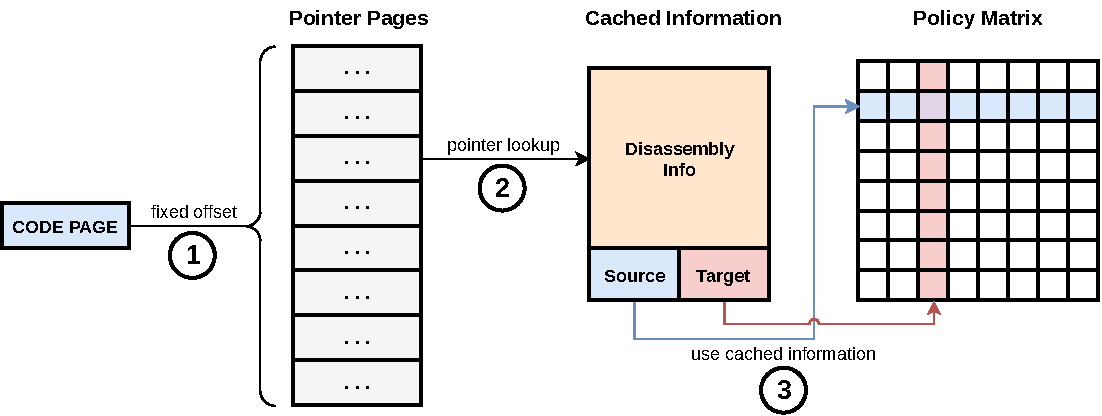
\includegraphics[width=1\columnwidth]{figs/matrix.pdf}
  \end{center}
\end{frame}

\begin{frame}[c]{P3: Stateful Policy}{}
  \begin{columns}
    \begin{column}{0.5\textwidth}
      \begin{itemize}
        \item Stateful policy is a fine-grained policy that also tracks {\bf state}
        \begin{itemize}
          \item Keep track of the call stack using a {\bf shadow stack}
        \end{itemize}

        \vspace{1.5em}
        \item Add extra rows to the policy matrix to store shadow stack

        \vspace{1.5em}
        \item Worker threads output a list of call and return addresses
        \begin{itemize}
          \item Compare calls and returns with shadow stack policy
        \end{itemize}
      \end{itemize}
    \end{column}
    \begin{column}{0.5\textwidth}
      \color{black}
      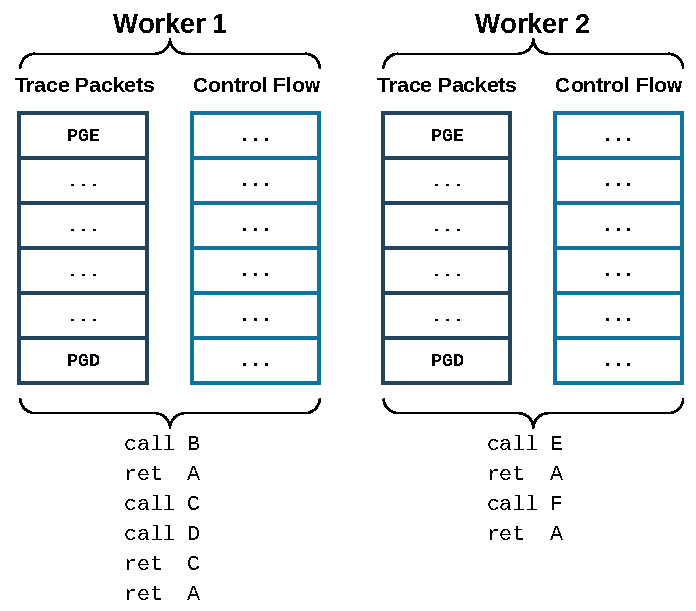
\includegraphics[width=1\columnwidth]{figs/stateful_policy.pdf}
    \end{column}
  \end{columns}
\end{frame}

\begin{frame}[c]{Problem: Sequential Reconstruction}{}
  \begin{itemize}
    \item Enforcing a shadow stack policy requires calls and rets to be {\bf in order}
    \begin{itemize}
      \item But Griffin is processing each trace in parallel
    \end{itemize}

    \vfill
    \item Solution: process traces in parallel and stitch together sequentially
    \begin{itemize}
      \item Order is preserved within a trace
      \item Just need to combine traces in sequence
    \end{itemize}

    \vfill
    \item This incurs some additional overhead due to the sequential phase
    \begin{itemize}
      \item But stateful policy is even more secure than fine-grained policy
    \end{itemize}
  \end{itemize}
\end{frame}

\begin{frame}[c]{P4: Combination Policy}{}
  \begin{itemize}
    \item A performance enhancement over stateful policy without sacrificing security
    \begin{itemize}
      \item Enforce stateful policy on back-edges (e.g.~returns)
      \item Enforce fine-grained policy on forward-edges (e.g.~calls)
    \end{itemize}

    \vfill
    \item Carlini \etal~\cite{carlini2015_cfi} recommend shadow stack enforcement on return addresses
    \begin{itemize}
      \item This helps mitigate ROP-style attacks by enforcing correct returns
      \item Benefits of a shadow stack for forward edges are less clear
      \item Therefore, Griffin can get away with shadow stack enforcement on back edges only
    \end{itemize}
  \end{itemize}
\end{frame}

\begin{frame}[c]{Problem: Support for JITed Languages}{}
  \begin{itemize}
    \item Problems arise when trying to support just-in-time compiled (JITed) applications
    \begin{itemize}
      \item Recall that this was one of Griffin's primary goals
      \item Some JIT compilers include optimizations that break Griffin
    \end{itemize}

    \vfill
    \item E.g.~Javascript under Firefox's Gecko engine
    \begin{itemize}
      \item Poisoning unmapped executable memory
      \item Incremental garbage collection
      \item OSR optimization breaks CFI
      \item Replacement of return instructions in switch table
    \end{itemize}

    \vfill
    \item In order to make it work, they had to manually patch Firefox's JIT compiler
    \begin{itemize}
      \item Can we reasonably expect to patch every single JIT compiler? (Of course not)
    \end{itemize}
  \end{itemize}
\end{frame}

\section{Griffin Evaluation}

\begin{frame}[c]{Evaluation: Performance Overhead}{}
  \begin{itemize}
    \item Performance evaluation consisted of micro- and macro-benchmarks
    \begin{itemize}
      \item Test Griffin's performance and memory overhead
      \item Allocated 6 worker threads and tested reduced numbers as well
    \end{itemize}

    \vfill
    \item SPEC CPU 2006 micro-benchmarks
    \begin{itemize}
      \item Commonly used to evaluate related work
      \item Intel PT without processing trace buffers as a control
      \item Evaluated overhead for coarse-grained, fine-grained, and combination policies
    \end{itemize}

    \vfill
    \item Real-world applications
    \begin{itemize}
      \item Firefox (with JIT compiler modifications)
      \item Nginx (web server)
      \item exim (email server)
      \item vsftpd (FTP daemon)
    \end{itemize}
  \end{itemize}
\end{frame}

\begin{frame}[c]{SPEC CPU 2006 Results}{}
  \begin{itemize}
    \item Average slowdowns:
    \begin{itemize}
      \item Coarse-grained: 5.6\% (Intel PT alone is 4.7\%)
      \item Fine-grained: 8.3\%
      \item Combination: 9.5\%
    \end{itemize}

    \vfill
    \item Worst-case overheads exceed 30\% (approaching impractical)

    \vfill
    \item Griffin is outperformed by some existing systems
    \begin{itemize}
      \item Some offer incomplete protection
      \item Others lack flexibility
    \end{itemize}

    \vfill
    \item Memory overhead is quite significant
    \begin{itemize}
      \item Hundreds of megabytes for complex applications
      \item Tens of megabytes for simple ones
    \end{itemize}
  \end{itemize}
\end{frame}

\begin{frame}[c]{Real-World Application Results}{}
  \begin{itemize}
    \item Performance impact on real-world applications is more modest
    \begin{itemize}
      \item About 12\% in the worst-case (Firefox)
      \item Negligible for vsftpd, exim, and Nginx
    \end{itemize}

    \vfill
    \item Reduction of worker threads has significant impact
    \begin{itemize}
      \item But the impact backs off significantly under larger work loads that slow the application down
    \end{itemize}

    \vfill
    \item I/O bound applications perform better under Griffin
    \begin{itemize}
      \item Many practical use cases for CFI are I/O bound applications
      \item E.g.~web servers, email clients, etc.
    \end{itemize}
  \end{itemize}
\end{frame}

\begin{frame}[c]{Optimizing Intel PT for Online CFI}{}
  {\bf Including Source Addresses in Intel PT}
  \begin{itemize}
    \item Perhaps the most obvious optimization
    \item Saves the need to do any reconstruction in fine-grained policy
    \begin{itemize}
      \item Stateful policy still requires some work, however
    \end{itemize}
    \item Trade-off between performance and memory
    \begin{itemize}
      \item Less work during online tracing, but traces would be larger
    \end{itemize}
    \item Could enable a toggle for offline use cases
  \end{itemize}

  \vfill
  {\bf Performance Improvements}
  \begin{itemize}
    \item With a manually modified trace, performance improves by 60--90\%
    \item Traces use about 19\% more memory
  \end{itemize}
\end{frame}

\begin{frame}[c]{Evaluation: Security}{}
  \begin{itemize}
    \item Used the RIPE benchmark to evaluate effectiveness
    \begin{itemize}
      \item 850 memory corruption / code reuse exploits
      \item The authors only managed to make 82 of these work
      \item Needed to disable ASLR and enable executable stack
    \end{itemize}
    \vfill
    \item Griffin was able to detect and stop all 82 exploits
    \begin{itemize}
      \item Coarse-grained and combination policy were equally effective
      \item Authors acknowledge that this is weak evidence
      \item Does not mean Griffin can stop every CFI attack
    \end{itemize}
  \end{itemize}
\end{frame}

\section{Discussion}

\begin{frame}[c]{Adoption Barriers}{}
  {\bf Performance / Memory Overhead}
  \begin{itemize}
    \item Would certainly be prohibitive in embedded systems
    \item Might be prohibitive for complex server workloads involving multiple concurrent processes
    \item Does increased flexibility justify extra memory/performance overhead over static solutions?
  \end{itemize}

  \vfill
  {\bf Incompatibilities with JIT Engines}
  \begin{itemize}
    \item The need to modify JIT engines for Griffin-compatibility is unrealistic
  \end{itemize}

  \vfill
  {\bf Other Limitations}
  \begin{itemize}
    \item Modifications to the scheduler are required to save per-thread information\\on context switches
    \item Griffin runs in ring 0, assumes a trusted kernel
  \end{itemize}
\end{frame}

\begin{frame}[c]{A Possible Attack}{}
  \begin{itemize}
    \item Something I came up with while reading about Griffin's policy switching strategy

    \vfill
    \item A quick recap:
    \begin{itemize}
      \item Griffin can switch to a coarser-grained policy when there are lots of\\outstanding trace buffers
      \item This serves as a proxy for the amount of performance bottlenecking
      \item Switching to a coarse-grained policy is less secure, but more performant
    \end{itemize}

    \vfill
    \item The attacker just needs to make the target run a lot of instructions quickly
    \begin{itemize}
      \item This is possible, since we assume the attacker can provide input to the target
      \item E.g.~modify scheduling priority, flood I/O bound program with small inputs
      \item This can force Griffin to switch to a more insecure policy
    \end{itemize}
  \end{itemize}
\end{frame}

%\begin{frame}[c]{Comparison with Related Work}{}
%
%\end{frame}
%
%\begin{frame}[c]{Alternative Hardware Tracing Solutions}{}
%
%\end{frame}

\begin{frame}[c]{Integration with eBPF?}{}
  \begin{itemize}
    \item eBPF is an observability framework for the Linux kernel
    \begin{itemize}
      \item Event-based tracing for userspace and kernelspace
      \item Integration with perf events subsystem
      \item Already support for some hardware-backed metrics, such as PMU counters
    \end{itemize}

    \vfill
    \item eBPF doesn't support Intel PT (yet)
    \begin{itemize}
      \item But adding support wouldn't be difficult
      \item Would just need a kernel helper to access the trace packets
    \end{itemize}

    \vfill
    \item Key advantage over using a kernel patch/module (Griffin style)
    \begin{itemize}
      \item Production safety
      \item Aggregate events in-kernel then hand off to userspace
      \item Easy integration with other userspace/kernelspace events
      \item System calls, function calls, scheduler run queue length, etc.
    \end{itemize}
  \end{itemize}
\end{frame}

\begin{frame}[c]{Discussion Questions}{}
  \begin{enumerate}
    \item Static CFI mechanisms like compile-time instrumentation can outperform Griffin, but often at the cost of flexibility. Do you think the flexibility argument justifies Griffin's adoption, despite performance concerns? Why or why not?

    \vfill
    \item Do you think the existence of Spectre variant 2 renders CFI mechanisms like Griffin pointless? Why or why not? (Recall: Spectre variant 2 involves executing Spectre gadgets via transient instructions.)

    \vfill
    \item Griffin's current threat model requires complete trust in the operating system kernel. Do you think this is justifiable? Would it be feasible to design such a system without this assumption?
  \end{enumerate}
\end{frame}

\appendix

\section{Backup Slides}

\section{References}

\nocite{*}
\begin{frame}[allowframebreaks, noframenumbering, plain]
  \frametitle{References}
  \sloppy%
  \printbibliography%
\end{frame}

\end{document}

% vim:syn=tex

